\documentclass[10pt,a4paper]{article}
\usepackage[T1]{fontenc}
\usepackage[utf8]{inputenc}
\usepackage{lmodern}
\usepackage[margin=20mm]{geometry}
\usepackage{microtype}
\usepackage{graphicx}
\usepackage{booktabs,tabularx,array,multirow}
\usepackage{amsmath,amssymb}
\usepackage{xcolor}
\usepackage[font=small,labelfont=bf]{caption}
\usepackage{enumitem}
\usepackage[section]{placeins}
\usepackage[hidelinks]{hyperref}
\graphicspath{{figures/}{../zuco_report/figures/}}
\setlist{nosep,leftmargin=*}
\newcolumntype{Y}{>{\raggedright\arraybackslash}X}

\title{Fuzzy Eye-Tracking Gates for Entropy-Based Fuzzy EEG Emotion Recognition\\[2pt]
\large Final Project Report: re-implementation of Farhadi Sedehi et al.\ (2024), proposed fuzzy gates M1 and M2,\\ and their evaluation on ZuCo~1.0 and SEED-IV}
\author{Soft Computing Project}
\date{November 2026}

\begin{document}
\maketitle

\begin{abstract}
\noindent
Farhadi Sedehi et al.\ (IEEE Access, 2024) recognise emotions from EEG with a hard eye-tracking gate, wavelet-band entropy features, mRMR feature selection, and a Sugeno fuzzy inference system whose rules are tuned by a genetic algorithm (GA). The gate keeps only the EEG windows in which a pupil feature is high, and the paper reports 94.4\% four-class accuracy on SEED-IV. No official code exists, so we re-implemented the full pipeline. We then proposed two softer gates: a fuzzy Low/Medium/High pupil gate (M1) and an adaptive temporal fuzzy gate with per-person breakpoints and smoothing over time (M2). We compared them with the paper's hard gate (M0) and with no gate. We evaluated on two real datasets: ZuCo~1.0 (12 participants, 4{,}430 sentences, text sentiment) and SEED-IV (15 participants $\times$ 3 sessions, 1{,}080 film-clip trials, 4 induced emotions), using a new PyTorch/CUDA implementation for the latter.
On ZuCo every model, including a logistic-regression reference, is at chance (33--35\%), so the dataset cannot discriminate between gates. On SEED-IV all models are well above chance (25\%). Per-person models on unseen clips reach 62--64\% for the fuzzy classifiers and 79.5\% for the logistic-regression reference. The no-gate model is as good as or slightly better than any gate. M1 and M2 do not improve on M0: they are 0.3--3.8 points lower, and M1 is significantly worse under 5-fold trial cross-validation ($p{=}0.017$). Under the paper's window-level split, the reference reaches 97.4\%, against 79.5\% when whole clips are held out. This indicates that the paper's 94.4\% is largely produced by its evaluation protocol. The project delivers a verified, reproducible implementation, an honest negative result for fuzzy gating, and a quantified explanation of the gap between published and realistic accuracy.
\end{abstract}

\tableofcontents

\section{Problem statement}
EEG-based emotion recognition is noisy: not every second of a recording reflects the emotion being studied. The baseline paper uses eye tracking to decide which EEG windows to trust, keeping windows in which pupil size, an index of arousal, is high, and discarding the rest. That hard threshold has three weaknesses. It throws away most of the data. It has no notion of ``partially relevant''. And its cut-off ignores differences between people.

\textbf{Objectives.}
\begin{enumerate}
  \item Re-implement the baseline pipeline (no official code is available).
  \item Replace the hard gate (M0) with fuzzy gates that weight every window by graded relevance: M1 (fuzzy Low/Medium/High) and M2 (adaptive per-person breakpoints plus temporal smoothing).
  \item Evaluate all gates on real EEG and eye-tracking data under leakage-free protocols and test whether the fuzzy gates improve accuracy.
\end{enumerate}
Multi-band probability fusion (former M3) and its combination with M2 (former M4) were dropped from the scope so that the gate is the only difference between models.

\section{The original method}
Fig.~\ref{fig:arch} shows the baseline pipeline. The paper evaluates it on SEED-IV and MAHNOB-HCI.
\begin{itemize}
  \item \textbf{Eye branch.} Eight eye features per 4-s window: fixation duration (mean, SD, max), fixation frequency, and pupil diameter X/Y (mean, SD). mRMR ranks them, and mean pupil diameter (Y) ranks first. Its maximum acts as the gating threshold: only EEG windows at high pupil values are used.
  \item \textbf{EEG branch.}
    \begin{itemize}
      \item Band-pass filtering and resampling to 128\,Hz.
      \item A db4 discrete wavelet transform splits the signal into five bands ($\delta$, $\theta$, $\alpha$, $\beta$, $\gamma$).
      \item Four nonlinear entropies are computed per window and channel: sample entropy (SampEn), permutation entropy (PermEn), symbolic dynamic entropy (SymbEn) and phase entropy (PhEn), with embedding $m{=}5$, $\tau{=}2$.
      \item mRMR selects three features (reported: PhEn-FP2, SampEn-T8, PermEn-T7).
    \end{itemize}
  \item \textbf{Classifier.} A zero-order Sugeno FIS with three levels per input (27 rule cells). Rules come from a lookup table (Wang--Mendel) and are tuned by a GA (population 27). One classifier is trained per band.
  \item \textbf{Reported results.} Five-fold cross-validation over pooled 4-s segments:
    \begin{itemize}
      \item SEED-IV: $\alpha$ 94.42\%, $\beta$ 93.02\%, $\gamma$ 89.80\%.
      \item MAHNOB-HCI: $\alpha$ 85.20\%, $\beta$ 82.92\%, $\gamma$ 79.05\%.
    \end{itemize}
\end{itemize}

\begin{figure}[h]
\centering
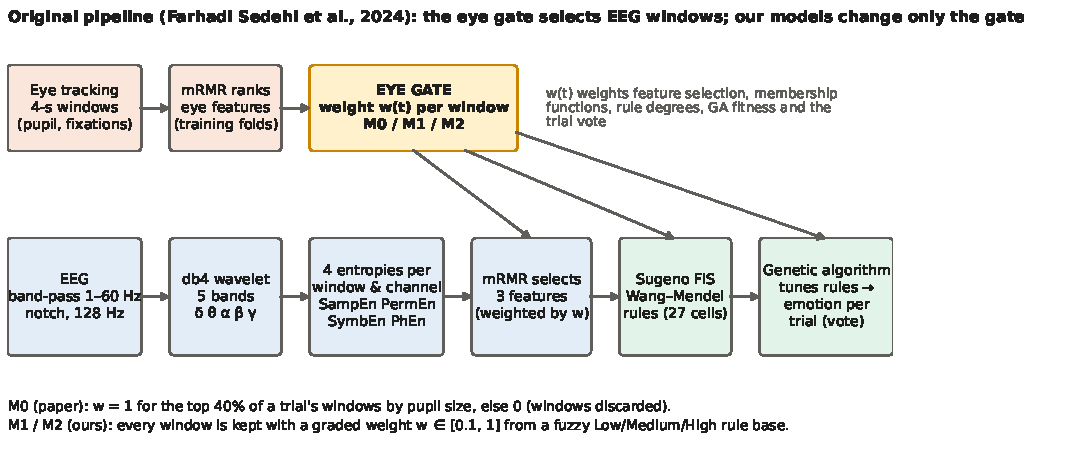
\includegraphics[width=\linewidth]{architecture.pdf}
\caption{Baseline architecture. The eye gate assigns a weight $w(t)$ to each 4-s window. In our implementation the weight enters every learning step, so a gate's effect is not limited to discarding windows.}\label{fig:arch}
\end{figure}

\section{Our contributions}
\subsection{Proposed gates}
All gates are label-free: they use only the eye signal. Let $v_t$ be the gate feature of window $t$; it is chosen by mRMR on the training fold. Fig.~\ref{fig:gates} plots each gate's weight as a function of the scaled pupil value.
\begin{itemize}
  \item \textbf{M0, hard gate (paper):} $w_t=\mathbf{1}[v_t\ge Q_{0.6}(\text{trial})]$. The top 40\% of each trial's windows get weight 1; the rest are dropped.
  \item \textbf{M1, fuzzy gate:}
    \begin{itemize}
      \item The signal is robust-scaled within each person or session: $\tilde z=\mathrm{clip}((v-P_5)/(P_{95}-P_5),0,1)$.
      \item Triangular Low/Medium/High memberships with breakpoints (0.2, 0.5, 0.8) fire three rules with outputs (0.1, 0.5, 1.0).
      \item The weight is the Sugeno weighted average $w=\sum_k\mu_k r_k/\sum_k\mu_k\in[0.1,1]$, so every window is kept.
    \end{itemize}
  \item \textbf{M2, adaptive temporal gate:}
    \begin{itemize}
      \item Missing pupil values are interpolated within the trial.
      \item The Low/Medium/High breakpoints are set to each person's own 20th/50th/80th percentiles (\emph{adaptive}).
      \item The weights are smoothed over neighbouring windows $(t{-}1,t,t{+}1)$ (\emph{temporal}). A causal variant uses only $(t{-}1,t)$.
    \end{itemize}
  \item \textbf{M1\,+\,temporal (ZuCo only):} M1 followed by M2's smoothing.
\end{itemize}
The weights enter weighted mRMR, membership-function fitting, Wang--Mendel rule degrees, GA fitness and the trial-level vote $\hat y=\arg\max_c\sum_t w_tP_t(c)/\sum_t w_t$.

\begin{figure}[h]
\centering
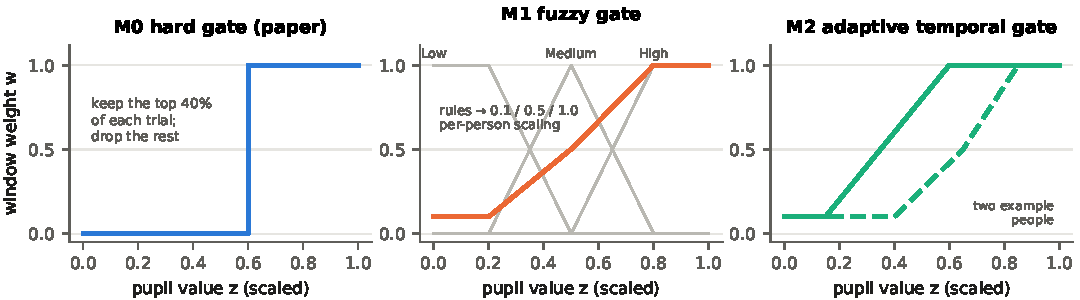
\includegraphics[width=\linewidth]{gates.pdf}
\caption{Window weight as a function of the scaled pupil value. M0 is a step. M1 is a graded fuzzy rule base. M2 adapts the breakpoints to each person (solid and dashed lines show two example people) and then smooths the weights over neighbouring windows.}\label{fig:gates}
\end{figure}

\subsection{Implementation}
\begin{itemize}
  \item \textbf{\texttt{gfer/} (CPU, NumPy):}
    \begin{itemize}
      \item the full pipeline;
      \item a ZuCo loader;
      \item the gates (\texttt{gates.py} for M0 and M1, \texttt{adaptive\_gate.py} for M2);
      \item the experiment runner and summaries.
    \end{itemize}
  \item \textbf{\texttt{gpu\_seed/} (GPU, PyTorch/CUDA):}
    \begin{itemize}
      \item SEED-IV layout discovery, plus a dataset inventory that also checks the labels against the dataset's ReadMe;
      \item batched GPU entropies, GPU mRMR, and a GA whose whole population is scored in one tensor operation;
      \item parallel workers and resumable, cached runs.
    \end{itemize}
    It reuses the gate code from \texttt{gfer}, so the models are identical across datasets. 16 unit tests check that the GPU code reproduces the NumPy reference.
  \item \textbf{Hardware:} SEED-IV ran on an NVIDIA RTX 4070 Laptop GPU. Feature extraction took about 37\,min in total (over two attempts); the 60 experiments took 20\,min.
\end{itemize}

\section{Datasets}
\begin{table}[h]
\centering\small
\caption{Datasets used.}\label{tab:data}
\begin{tabularx}{\linewidth}{@{}lYY@{}}
\toprule
 & ZuCo 1.0, task 1 & SEED-IV \\
\midrule
Stimulus & Reading movie-review sentences & Watching emotional film clips \\
Label & Text sentiment (neg./neutral/pos.), not the reader's emotion & Induced emotion (neutral/sad/fear/happy) \\
Participants, trials & 12; 4{,}430 sentences (2--30\,s) & 15 $\times$ 3 sessions; 1{,}080 clips (roughly 1.5--4\,min) \\
EEG & EGI 128 net, 19 channels at 10--20 positions, 500\,Hz $\to$ 128\,Hz & 62 channels, 200\,Hz $\to$ 128\,Hz \\
Eye tracking & EyeLink pupil area, fixations & 31 features per 4-s window (eye\_feature\_smooth) \\
Windows & 1\,s (23{,}683) & 4\,s (37{,}575) \\
Chance & 33.3\% & 25\% \\
Verified & Sentence/label alignment on all 46 control markers & 15 subjects $\times$ [1,2,3]; 200\,Hz; labels identical to the dataset ReadMe \\
\bottomrule
\end{tabularx}
\end{table}

\section{Evaluation protocols}
Every label-dependent step (mRMR, membership functions, rules, GA, gate-feature choice) is fitted on training data only. Results are the mean of 3 seeds.
\begin{itemize}
  \item \textbf{Per-person (\texttt{within}, SEED-IV):} for each person, 5-fold over their 72 trials. Test clips are clips this person's model never saw.
  \item \textbf{5-fold over trials:} all people pooled; whole trials held out.
  \item \textbf{Leave-one-subject-out (LOSO):} the test person is never seen in training.
  \item \textbf{Paper protocol (SEED-IV):} 5-fold over pooled 4-s windows. Windows of the same clip appear in both training and test, so this is reported only for comparison with the paper.
  \item \textbf{Statistics:}
    \begin{itemize}
      \item one-sided binomial test against chance;
      \item exact McNemar test between two models on the same trials;
      \item Wilcoxon signed-rank test over participants (LOSO).
    \end{itemize}
\end{itemize}

\section{Defects found and fixed}
The pipeline was first developed on synthetic data. Running it on real data exposed the problems in Table~\ref{tab:fixes}. Every correction was applied identically to all models, and each was decided from diagnostics, never from test accuracy.

\begin{table}[h]
\centering\small
\caption{Defects and corrections.}\label{tab:fixes}
\begin{tabularx}{\linewidth}{@{}p{4.1cm}YY@{}}
\toprule
Problem & Evidence & Correction\\
\midrule
Entropy settings on 1-s windows (ZuCo) & SampEn returned a constant in 57--94\% of $\alpha/\beta/\gamma$ windows & $m{=}3,\tau{=}1$; SampEn $m{=}2$ (SEED-IV keeps the paper's $m{=}5,\tau{=}2$ on 4-s windows)\\
Flat reference channel (Cz) & mRMR picked its constant features & Constant features excluded; Cz dropped\\
GA collapsed to one rule & ``Always neutral'' maximised accuracy\,+\,coverage & Balanced-accuracy fitness\\
Minority class had no rules & Wang--Mendel gave 26/27 cells to the larger classes & Class-balanced training weights\\
M1 nearly a copy of M0 & Within-trial scaling gave $r{=}0.81$ with M0 & Per-person scaling ($r{=}0.28$)\\
Old M2 baseline had no effect & Cancelled by within-trial rescaling & M2 rewritten\\
Windows encoding; 1.5\,GB IPC messages; CUDA wheels & Crashes on the GPU laptop & UTF-8 output; temporary files; cu128 PyTorch build\\
\bottomrule
\end{tabularx}
\end{table}

\section{Results on ZuCo 1.0}
\begin{figure}[h]
\centering
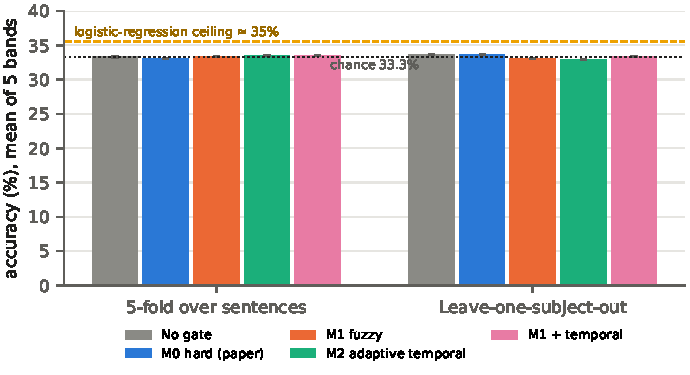
\includegraphics[width=0.72\linewidth]{zuco_results.pdf}
\caption{ZuCo: accuracy averaged over the five bands. All models are at chance. Even a logistic regression on all features reaches only about 35\%.}\label{fig:zuco}
\end{figure}

\begin{table}[h]
\centering\small
\caption{ZuCo: accuracy (\%) averaged over the five bands, and each proposed gate minus M0 over 15 band$\times$seed runs.}\label{tab:zuco}
\begin{tabular}{@{}lcccccc@{}}
\toprule
 & No gate & M0 & M1 & M2 & M1+temporal & LogReg ref.\\
\midrule
5-fold over sentences & 33.3 & 33.0 & 33.3 & 33.4 & 33.5 & 35.2\\
LOSO & 33.7 & 33.6 & 33.1 & 33.0 & 33.4 & 35.5\\
\midrule
$\Delta$ vs M0, 5-fold (runs ahead) & & & $+0.32$ (11/15) & $+0.44$ (10/15) & $+0.47$ (13/15) & \\
$\Delta$ vs M0, LOSO (runs ahead) & & & $-0.52$ (4/15) & $-0.62$ (3/15) & $-0.23$ (7/15) & \\
\bottomrule
\end{tabular}
\end{table}

No overall difference is significant (Wilcoxon over participants, all $p>0.1$). ZuCo labels the sentiment of the text, not an emotion felt by the reader, and the EEG and pupil features carry almost no sentiment information. ZuCo therefore cannot test the gates. It served to debug and verify the pipeline on real data.

\section{Results on SEED-IV}
\begin{figure}[h]
\centering
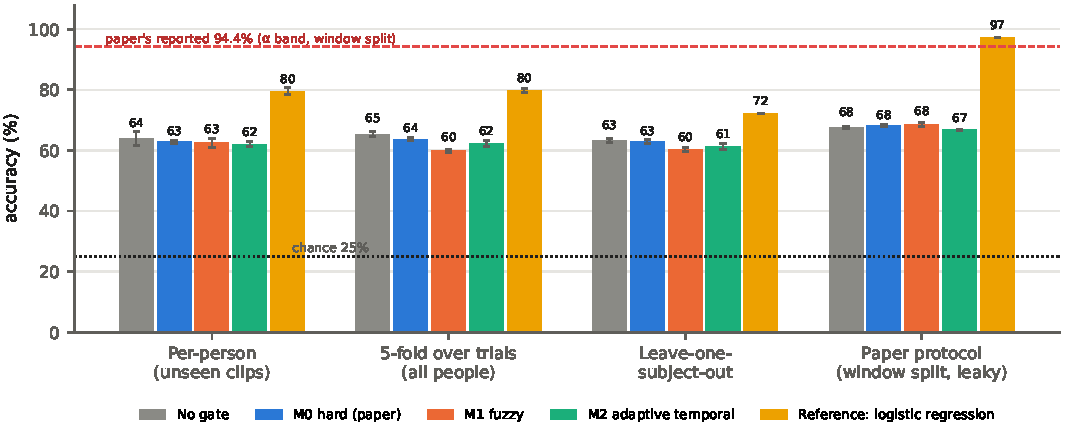
\includegraphics[width=\linewidth]{seed_results.pdf}
\caption{SEED-IV accuracy (mean $\pm$ SD over 3 seeds) for each protocol. All models are far above chance (25\%). The window split (right) inflates the reference model to 97.4\%, close to the paper's reported 94.4\%.}\label{fig:seed}
\end{figure}

\begin{table}[h]
\centering\small
\caption{SEED-IV accuracy (\%), mean $\pm$ SD over 3 seeds. Features: DE\,+\,4 entropies\,+\,eye, all bands pooled, 4 fuzzy inputs. All values are far above chance (one-sided binomial $p<0.05$ for every trial-level cell).}\label{tab:seed}
\begin{tabular}{@{}lccccc@{}}
\toprule
Protocol & No gate & M0 hard & M1 fuzzy & M2 adaptive & LogReg ref.\\
\midrule
Per-person (unseen clips) & \textbf{64.0} $\pm$ 2.2 & 62.9 $\pm$ 0.5 & 62.5 $\pm$ 1.4 & 62.1 $\pm$ 0.7 & 79.5 $\pm$ 1.2\\
5-fold over trials & \textbf{65.4} $\pm$ 0.7 & 63.8 $\pm$ 0.6 & 59.9 $\pm$ 0.5 & 62.3 $\pm$ 1.0 & 79.8 $\pm$ 0.6\\
Leave-one-subject-out & \textbf{63.3} $\pm$ 0.7 & 62.8 $\pm$ 0.6 & 60.2 $\pm$ 0.7 & 61.3 $\pm$ 1.1 & 72.0 $\pm$ 0.0\\
Paper protocol (window split) & 67.6 $\pm$ 0.4 & 68.2 $\pm$ 0.3 & \textbf{68.4} $\pm$ 0.7 & 66.7 $\pm$ 0.2 & 97.4 $\pm$ 0.0\\
\bottomrule
\end{tabular}
\end{table}

\begin{table}[h]
\centering\small
\caption{SEED-IV: proposed gates minus M0 (points), with the exact McNemar test (seed 0, pooled trials) and, for LOSO, the Wilcoxon test over the 15 participants.}\label{tab:seeddelta}
\begin{tabular}{@{}lcccc@{}}
\toprule
 & Per-person & 5-fold trials & LOSO & Paper protocol\\
\midrule
M1 $-$ M0 & $-0.34$ ($p{=}0.37$) & $\mathbf{-3.83}$ ($p{=}0.017$) & $-2.65$ ($p{=}0.12$; Wilcoxon 0.37, 5/15 helped) & $+0.24$\\
M2 $-$ M0 & $-0.77$ ($p{=}0.67$) & $-1.48$ ($p{=}0.62$) & $-1.54$ ($p{=}0.18$; Wilcoxon 0.35, 6/15 helped) & $-1.45$\\
\bottomrule
\end{tabular}
\end{table}

\begin{table}[h]
\centering\small
\caption{SEED-IV per-class recall (\%) in the per-person protocol.}\label{tab:recall}
\begin{tabular}{@{}lcccc@{}}
\toprule
Model & Neutral & Sad & Fear & Happy\\
\midrule
No gate & 74.9 & 56.3 & 77.4 & 47.2\\
M0 hard & 71.9 & 55.2 & 77.0 & 47.4\\
M1 fuzzy & 80.2 & 54.8 & 72.3 & 42.7\\
M2 adaptive & 79.6 & 54.8 & 71.7 & 42.2\\
LogReg ref. & 90.6 & 75.1 & 81.4 & 71.0\\
\bottomrule
\end{tabular}
\end{table}

\begin{figure}[h]
\centering
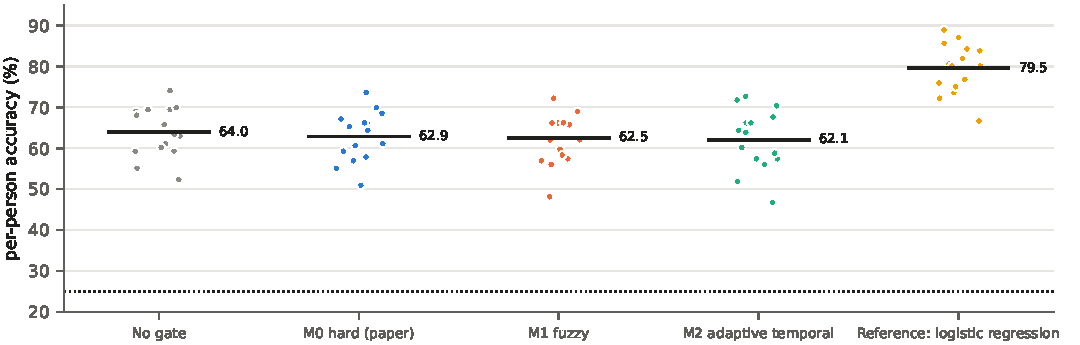
\includegraphics[width=\linewidth]{seed_persubject.pdf}
\caption{SEED-IV, per-person protocol: accuracy of each of the 15 participants (dots) and the mean (bar). The spread between people (about 47--74\% for the fuzzy models) is far larger than the differences between gates.}\label{fig:persub}
\end{figure}

\paragraph{Findings.}
\begin{enumerate}
  \item \textbf{The pipeline works on emotion data.} Fuzzy models reach 60--68\% on four classes (chance 25\%) with only four inputs and 29--48 readable rules.
  \item \textbf{Gating does not help.} The no-gate model matches or beats every gate under all three honest protocols. M1 and M2 are 0.3--3.8 points below M0. The only significant difference favours M0 (M1, 5-fold, $p{=}0.017$). M1 and M2 shift recall towards neutral at the expense of sad and happy (Table~\ref{tab:recall}, and more strongly in the pooled protocols).
  \item \textbf{The fuzzy classifier is capacity-limited.} The logistic-regression reference on all features is 15--17 points higher (79.5\% per person). With pooled people, the fuzzy models selected only DE and eye features, never the paper's entropies. Per person the mix was about 40\% DE, 35\% eye and 25\% entropy.
  \item \textbf{The window split explains the paper's 94\%.} The same reference model scores 97.4\% with the paper's window-level split but 79.5\% when whole clips are held out. Neighbouring windows of one clip are nearly identical, and SEED-IV's DE and eye features are temporally smoothed, so a window split largely tests clip recognition.
\end{enumerate}

\section{Discussion}
\textbf{Why the fuzzy gates do not improve accuracy.} A gate helps only if the windows it down-weights carry less class information than those it keeps. On SEED-IV, all windows of a clip appear similarly informative: the no-gate model is best. M0's discarding and M1/M2's re-weighting therefore remove useful evidence rather than noise. The pupil is also driven by screen luminance, which differs between film clips, so ``high pupil'' does not reliably mark ``emotional'' windows.

\textbf{What the fuzzy gates do offer.} They keep every window, replace an arbitrary hard cut-off with an interpretable three-rule system, and adapt to each person (M2). They cost little accuracy: within one point of M0 per person.

\textbf{Cross-person protocols.} All SEED-IV participants watched the same clips in the same order. In 5-fold-over-trials and LOSO, a test clip has therefore been seen, from other people, during training. Stimulus-driven features, especially pupil and other eye features, can then help identify the clip. This plausibly explains why the reference model still reaches 72\% across people. The per-person protocol, where each test clip is new, is the cleanest estimate. We report it as primary, but we could not test this confound directly.

\section{Limitations}
\begin{itemize}
  \item \textbf{Only the improved feature set was run on SEED-IV.} The paper-faithful run (entropy features only, three inputs, one band at a time) was implemented but not executed, so a per-band replication of the paper's numbers is not available.
  \item \textbf{Eye features are identified by column index only.} SEED-IV provides 31 unnamed eye features. The gate most often chose column~0 (56\% of folds).
  \item \textbf{Gate parameters were fixed in advance, not tuned.} We used three seeds.
  \item \textbf{ZuCo's task is not emotion recognition.}
\end{itemize}

\section{Conclusion and future work}
We re-implemented the eye-gated fuzzy EEG pipeline and verified it end to end on two real datasets. We proposed fuzzy (M1) and adaptive temporal (M2) eye gates and evaluated them rigorously. On SEED-IV the fuzzy classifiers recognise four emotions far above chance (62--64\% per person on unseen clips), but neither proposed gate improves on the paper's hard gate. Gating as such does not improve on using all windows. The paper's 94\% is reproduced only under its window-level split; holding out whole clips lowers accuracy substantially.
\begin{itemize}
  \item \textbf{Future work: interpretability.} Use the fuzzy gate as an interpretability tool rather than an accuracy tool.
  \item \textbf{Future work: classifier capacity.} Use more fuzzy inputs or hierarchical rule bases to close the gap to the 79.5\% reference.
  \item \textbf{Future work: the paper-faithful run.} Run the paper-faithful SEED-IV preset for a per-band replication.
  \item \textbf{Future work: luminance.} Control for screen luminance in the pupil signal.
\end{itemize}

\appendix
\section{Reproducibility}
\begin{small}
\begin{verbatim}
# ZuCo (CPU):   python scripts/download_zuco.py --out data/zuco --jobs 6
#               python -m gfer.zuco --src data/zuco --out data/zuco_npz
#               python -m gfer.compare --datasets data/zuco_npz --protocols trial,loso --seeds 0,1,2
# SEED-IV (GPU, branch seed-iv-gpu):
#               pip install torch --index-url https://download.pytorch.org/whl/cu128
#               python -m gpu_seed --root <SEED-IV folder> --preset improved
# Figures:      python manuscript/final_project_report/make_figures.py
\end{verbatim}
\end{small}
\begin{itemize}
  \item \textbf{Results:}
    \begin{itemize}
      \item SEED-IV: \texttt{gpu\_seed/results/improved/}
      \item ZuCo: \texttt{results/zuco\_final\_m0m1/}, \texttt{results/zuco\_m2/}, \texttt{results/zuco\_combo/}
    \end{itemize}
  \item \textbf{Every number in this report:} \texttt{seed\_stats.json} and \texttt{../zuco\_report/stats.json}.
  \item \textbf{Full project description:} \texttt{FINAL\_REPORT.md} at the repository root.
\end{itemize}

\section*{References}
\begin{small}
\begin{itemize}
  \item J.~Farhadi Sedehi, N.~Jafarnia Dabanloo, K.~Maghooli, A.~Sheikhani, ``Recognition of emotional categories using mined fuzzy rules from electroencephalogram signals with gated eye track data approach,'' \emph{IEEE Access} 12:118122--118140, 2024. doi:10.1109/ACCESS.2024.3430934.
  \item W.-L.~Zheng, W.~Liu, Y.~Lu, B.-L.~Lu, A.~Cichocki, ``EmotionMeter: a multimodal framework for recognizing human emotions,'' \emph{IEEE Trans.\ Cybernetics} 49(3):1110--1122, 2019 (SEED-IV). doi:10.1109/TCYB.2018.2797176.
  \item N.~Hollenstein et al., ``ZuCo, a simultaneous EEG and eye-tracking resource for natural sentence reading,'' \emph{Scientific Data} 5:180291, 2018. doi:10.1038/sdata.2018.291.
\end{itemize}
\end{small}
\end{document}
